\documentclass[a4paper,12pt]{report}

\usepackage[polish]{babel}
\usepackage[utf8]{inputenc}
\usepackage{polski}
\usepackage[T1]{fontenc}
\frenchspacing 
\usepackage{indentfirst}
\usepackage{graphicx}
\usepackage{listings}
\lstset{
  xleftmargin=10pt,
  framexleftmargin=10pt,
  framexrightmargin=5pt,
  showspaces=false,
  showstringspaces=false,
  breaklines=true
  inputencoding=utf8x,
  stringstyle=\ttfamily,
  basicstyle=\small,
  prebreak=\raisebox{0ex}[0ex][0ex]{\ensuremath{\hookleftarrow}},
  literate={ą}{{\k{a}}}1
             {Ą}{{\k{A}}}1
             {ę}{{\k{e}}}1
             {Ę}{{\k{E}}}1
             {ó}{{\'o}}1
             {Ó}{{\'O}}1
             {ś}{{\'s}}1
             {Ś}{{\'S}}1
             {ł}{{\l{}}}1
             {Ł}{{\L{}}}1
             {ż}{{\.z}}1
             {Ż}{{\.Z}}1
             {ź}{{\'z}}1
             {Ź}{{\'Z}}1
             {ć}{{\'c}}1
             {Ć}{{\'C}}1
             {ń}{{\'n}}1
             {Ń}{{\'N}}1
}

\author{Marcin Baliński}
\title{Testowo Zorientowane Metodyki Wytwarzania Oprogramowania}

\begin{document}
	\maketitle
	\tableofcontents
	% Copyright 2011, Marcin Baliński

\nocite{ruby_way}
\nocite{rails_guides}
\nocite{polish_ruby_forum}

\chapter[Wstęp]{Wstęp}
  Metodyka to ustandaryzowane dla wybranego obszaru podejście do rozwiązywania problemów. Praca ta ma na celu szczegółowe omówienie dwóch najbardziej znanych metodyk rozwoju oprogramowania w oparciu o testy: \emph{Test Driven Development} oraz \emph{Behavior Driven Development} wraz ze szczegółowym opisem narzędzi wspomagających rozwój oprogramowania napisanego w języku \emph{Ruby} w zgodzie z tymi metodykami.
  
  Kolejnym nie mniej ważnym celem jest pokazanie jak niezmiernie istotne jest testowanie kodu. Opisane zostaną zarówno problemy wynikające z braku odpowiedniego pakietu testów jak i korzyści płynące z prawidłowego wdrożenia testowo zorientowanych metod rozwoju do projektu informatycznego. Nie zabraknie również wskazówek odnośnie najlepszych praktyk jakie należy stosować przy wdrażaniu testowo zorientowanych metodyk.
  
  We wstępie znajduje się ogólny opis idei testowania oprogramowania oraz omówienie najpowszechniejszych problemów i trudności związanych z procesem jego rozwoju. Kolejne dwa rozdziały to szczegółowy opis technik \emph{Test Driven Development}, \emph{Behavior Driven Development} oraz narzędzi wspomagających ich wdrożenie w projektach tworzonych przy pomocy języka \emph{Ruby}. Rozdział czwarty to studium przypadku - praktyczny opis tego jak w praktyce wygląda \emph{Behavior Driven Development} na przykładzie rozwoju projektu Open Source. Rozdział czwarty kończy się podsumowaniem zalet testowo zorientowanych metodyk rozwoju oprogramowania oraz czynników determinujących powodzenie ich wdrożenia wraz z krótkimi wnioskami.
  
	\section{Problemy napotykane w procesie wytwarzania oprogramowania}
	  Na każdy projekt informatyczny można patrzeć z różnych perspektyw. Praca ta omawia techniczny aspekt rozwoju oprogramowania w wybranym języku programowania, zaczynając od przybliżenia najczęstszych problemów napotykanych podczas tej fazy.
	  
	  Rozwój oprogramowania nie jest rzeczą trywialną. Po dogłębnej analizie potrzeb, wybraniu narzędzi, które posłużą do budowy systemu następuje faza implementacji, której trudność zależy od wielu czynników takich jak:
	  
	  \begin{description}
	    \item[Rodzaj wybranych narzędzi] Czy wybrane środki techniczne takie jak język programowania lub zestaw zewnętrznych bibliotek nadają się do rozwiązania tego typu problemu?
	    \item[Stopień skomplikowania systemu]
	    \item[Stopień integracji systemu] Czy łatwo oddzielić od siebie poszczególne wewnętrzne funkcje systemu? Czy konieczna jest integracja z zewnętrznym oprogramowaniem?
	    \item[Wielkość zespołu programistów]
	    \item[Stopień technicznej świadomości uczestników projektu] Wpływa na jakość komunikacji z programistami.
	  \end{description}
	  
	  Powyższe czynniki wpływają bezpośrednio na problemy, które pojawiają się podczas implementacji systemu. Rozwojowi oprogramowania najczęściej towarzyszą problemy takie jak:
	  
	  \begin{description}
  	  \item[Wzrost stopnia skomplikowania bazy kodu]
  	    Kod staje się coraz bardziej skomplikowany i trudniejszy w utrzymaniu. Wynika to często z braku ustalonych konwencji, polityki włączania do projektu zewnętrznych rozwiązań lub słabej komunikacji w zespole programistów.
  	  \item[Niepotrzebny wzrost stopnia integracji]
  	    Łamanie zasady modułowego tworzenia oprogramowania. Poszczególne części systemu są ze sobą coraz bardziej związane i znacząco na siebie wpływają. Powoduje to sytuację, w której usterka w jednym module powoduję awarię w kilku innych częściach systemu.
  	  \item[Trudność w utrzymaniu systemu zgodnie z dostarczoną specyfikacją]
  	    Wynikająca z niewłaściwej komunikacji lub z wcześniejszych błędów.
  	\end{description}
	
	\subsubsection{}
	Dokładniejszą analizę przyczyn i skutków problemów napotykanych podczas procesu rozwoju oprogramowania znaleźć można między innymi w takich pozycjach jak \cite{pragmatic_programmer} oraz \cite{rspec_book}.  W świetle tych informacji logicznym wydaje się wprowadzenie narzędzia kontroli, dzięki któremu można by upewnić się co do jakości dostarczonych rozwiązań a także zminimalizować ryzyko pojawienia się podobnych problemów w przyszłości. Jednym z takich narzędzi są testy oprogramowania.
	  
	\section{Testowanie oprogramowania}
	  \subsection{Wady manualnego testowania}
  	  Testowanie oprogramowania może odbywać się w sposób manualny lub automatyczny. Testy manualne przeprowadzane są przez żywego testera, który korzystając z oprogramowania krok po kroku sprawdza jego zgodność ze specyfikacją a następnie wskazuje i opisuje ewentualne braki lub błędy. Każda nowa funkcjonalność lub poprawka wprowadzona do oprogramowania wymaga osobnej sesji z udziałem testera. 
	  
  	  Podejście manualne ma wiele wad, wśród których do najważniejszych należą:
	  
  	  \begin{itemize}
  	    \item Konieczność dogłębnego zrozumienia założeń projektu przez osobę odpowiedzialną za testowanie
  	    \item Trudność związana z koniecznością zidentyfikowania i przetestowania jak największej liczby możliwych przypadków użycia oprogramowania
  	    \item Czasochłonność: każda nowa funkcjonalność lub poprawka wymaga osobnej sesji testowania
  	   	\item Wysokie koszty pracy testera
  	   	\item Ogromna trudność zastosowania w wysoce specjalistycznych projektach
  	   	\item Brak możliwości dokładnego przetestowania szczegółów implementacji danej funkcjonalności
  	  \end{itemize}
	  
  	  Waga powyższych niedogodności rośnie wykładniczo wraz ze wzrostem poziomu skomplikowania oprogramowania dlatego też manualne testowanie sprawdza się w zasadzie tylko w projektach o małej złożoności. W innych przypadkach istnieje potrzeba uzupełnienia lub zastąpienia żywego testera przez testy automatyczne.
	  
	  \subsection{Testy automatyczne}
	    Automatyzacja procesu testowania odbywa się poprzez zastąpienie testera oprogramowaniem, które przejmie jego rolę. Automatyczne metody testowania umożliwiają sprawdzenie działania kodu programu jak również graficznego interfejsu użytkownika.
	    \subsubsection{Testowanie kodu}
	    
	      W procesie tym testujemy szczegóły implementacji systemu. Oprócz kodu potrzebnego do zrealizowania danej funkcjonalności programiści piszą również testy weryfikujące jej implementację. Testy takie mogą mieć różne funkcje, przykładowo:
	      
	      \begin{description}
	        \item[Testy jednostkowe] Sprawdzają pojedynczy, niepodzielny element implementacji taki jak metoda lub funkcja
	        \item[Testy integracyjne] Sprawdzają interakcję między składowymi elementami systemu
        \end{description}
        
        Celem testu może być sprawdzenie wyniku działania danej części kodu, może być nim również chęć upewnienia się, że wynik działania osiągnięty jest w konkretny sposób. Dla przykładu testując funkcję, której zadaniem jest wyświetlić na ekranie monitora napis \emph{Witaj Świecie!} możliwe jest, że prócz samego faktu pojawienia się treści na ekranie chcemy również upewnić się, że do jej wyświetlenia użyta została jakaś konkretna metoda pochodząca z biblioteki standardowej. Jest to duża przewaga w stosunku to manualnego testowania oprogramowania, które nie daje nam takiej możliwości kontrolowania procesów prowadzących do widzialnych rezultatów.

        W chwili obecnej istnieją dziesiątki gotowych narzędzi pozwalających testować kod napisany w każdym szerzej używanym języku programowania. Ich używanie należy do podstaw każdej nowoczesnej metodyki prowadzenia projektów informatycznych.
        
      \subsubsection{Testowanie interfejsu użytkownika}
        
        Istnieje szereg narzędzi pozwalających testować zachowanie, oraz wygląd interfejsów użytkownika, ich działanie opiera się najczęściej na nagrywaniu i późniejszym odtwarzaniu testowanych interakcji oraz porównywaniu ich rezultatów z naszymi oczekiwaniami. W taki sposób można testować tradycyjne aplikacje, jak również aplikacje www działające w przeglądarce\footnote{w tym  przypadku szczegóły działania narzędzi testujących są inne, interfejs użytkownika jest bowiem najczęściej zdefiniowany przez znaczniki HTML.}
        
        W kwestii testowania interfejsu użytkownika przewaga automatycznych testów nie jest już tak druzgocąca jak w przypadku testowania kodu, jednak i tutaj jesteśmy w stanie znacząco skorzystać na automatyzacji, zyskiem jest przede wszystkim czas oraz zerowy koszt powtórzenia testu.
        
      \subsubsection{}

        Decydując się na automatyzacje procesu testowania oprogramowania należy pamiętać, że nadal kluczowym elementem jest konieczność dogłębnego zrozumienia specyfikacji oprogramowania przez osobę odpowiedzialną za pisanie testów. Równie ważnym wymogiem jest to, że pakiet testów powinien być kompletny, to znaczy pokrywać wszystkie kluczowe elementy systemu. Im większy procent kodu pokryty jest testami tym lepiej. Oznacza to również, że każdy nowy kod musi być dostarczony wraz z odpowiednimi testami.
        
        Jeśli spełnimy te warunki proces utrzymania oprogramowania stanie się dużo łatwiejszy. Oto niektóre z korzyści:
        
         \begin{itemize}
     	    \item Mamy pewność, że system działa zgodnie z założeniami
     	    \item Proces modyfikacji oprogramowania staje się łatwiejszy i bezpieczniejszy: jeśli nowy kod spowoduje defekt w którejś z bieżących funkcjonalności zostaniemy o tym niezwłocznie poinformowani przez nie przechodzący test
     	  \end{itemize}
     	  
     	  Na temat automatyzacji procesu testowania oprogramowania napisano ogromną ilość książek oraz artykułów. Dobrym punktem startu dla tych, którzy chcieliby zgłębić temat będzie strona wikipedii\footnote{http://en.wikipedia.org/wiki/Test\_automation} \nocite{wiki_test_automation} poświęcona temu tematowi.


	% Copyright 2011, Marcin Baliński

\chapter[Test Driven Development]{Test Driven Development}
  \section{Czym jest TDD?}
    Test Driven Development jest praktyką, według założeń której każda modyfikacja systemu poprzedzona jest stworzeniem odpowiedniego testu opisującego tą modyfikację. Programista zaczyna od napisania testu, który z naturalnych przyczyn (testowany kod nie istnieje a tym etapie) daje wynik negatywny. Następnie napisany zostaje właściwy kod, którego zachowanie zgodne jest z testowanym. Kiedy testy przechodzą można wprowadzić ewentualne poprawki.
    Proces rozwoju oprogramowania w zgodzie z filozofią TDD składa się z wielu takich cyklów, które zobrazować można diagramem:
    
    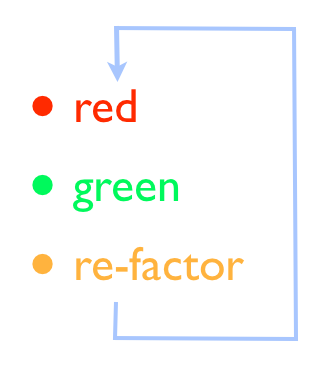
\includegraphics[width=75mm]{images/tdd_red_green_refactor.png}
    
    \begin{description}
      \item[Red] Pierwszy etap cyklu otrzymał swoją nazwę ze względu na to, że w większości środowisk służących do testowania oprogramowania testy, które zakończyły się niepowodzeniem oznaczane są czerwony kolorem. Etap ten polega na napisaniu testu przed rozpoczęciem implementacji właściwej funkcjonalności oraz na uruchomieniu go. Należy upewnić się, że w tym momencie test zakończy się niepowodzeniem - daje to pewność, że faktycznie testujemy nowe zachowanie, którego w tym momencie system jeszcze nie obsługuje a także że ewentualna przypadkowa modyfikacja tego zachowania zawsze zostanie wykryta przez nieprzechodzący test.
      \item[Green] Drugi etap polega na zaprogramowaniu zachowania opisanego wcześniejszym testem. Programista piszę tylko tyle kodu, aby spełnić warunki testu po czym uruchamia ponownie cały zestaw testów. Uruchomienie tylko ostatniego testu związanego z napisanym kodem jest nie wystarczające - może okazać się, że nasze ostatnie zmiany modyfikują bezpośrednio lub pośrednio wiele obszarów aplikacji. Jak wskazuje nazwa, etap ten powinien zakończyć się gdy wszystkie do tej pory stworzone testy przechodzą pozytywnie.
      \item[Re-factor] Ostatni etap polega na jakościowej modyfikacji kody. W tym momencie programista powinien skupić się na usunięciu wszelkich zbędnych powtórzeń, uproszczeniu implementacji czy też dopracowaniu użytego nazewnictwa zmiennych lub metod. Etap ten nie pociąga za sobą żadnych zmian w sposobie działania oprogramowania, jest jednak równie ważny jak poprzednie, dobry jakościowo kod jest łatwiejszy w utrzymaniu i modyfikacji.
    \end{description}
    
    Opisane powyżej iterację powinny być jak najprostsze. Oznacza to, że każdą implementowaną funkcjonalność należy podzielić na jak najmniejsze części i wykonywać pełen zestaw powyższych kroków dla każdej z nich. Idealna sytuacja to taka, w której pojedynczy test sprawdza tylko jedną rzecz.

  \subsection{Główne zasady TDD}
    \paragraph{Zacznij od testu}
      Test powinien być napisany zanim zacznie się implementacja funkcjonalności. Takie podejście gwarantuje, że będziemy mieli pełen zestaw testów opisujących każdą funkcję systemu. Inną zaletą jest konieczność dokładnego przemyślenia szczegółów implementacji jeszcze przed jej rozpoczęciem.
    \paragraph{Zaraz po napisaniu nowe testy powinny dawać negatywny wynik}
      Daje to pewność, że testy faktycznie spełniają swoją funkcję, oraz każda degradacja funkcjonalności będzie sygnalizowana nieprzechodzącym testem.
      
      Dużo więcej na temat historii, filozofii oraz zasad Test Driven Development znaleźć można w książce \emph{The RSpec Book}\footnote{\cite{rspec_book}}
      
  \subsection{Przykładowe iteracja TDD}
    Przypuśćmy, że pracujemy nad oprogramowaniem sportowej tablicy wyników. Naszym aktualnym zadaniem jest napisanie metody, która na wejściu otrzymuje nazwy dwóch drużyn sportowych, zwraca zaś łańcuch składający się z nazw tych drużyn połączonych łańcuchem " vs ". Oprogramowanie napisane jest w języku Ruby, do testowania użyjemy biblioteki RSpec.
    
    Praca rozpoczyna się od napisania testu opisującego pożądane zachowanie. W naszym wypadku może on wyglądać tak: 
    
    \lstinputlisting[language=ruby]{examples/code/ch02/01.rb}

    Dokładny opis budowy testu zawarty jest w podrozdziale \emph{Narzędzia wspierające TDD dostępne dla języka Ruby} i nie będę go tutaj powielał. Chciałbym jednak zwrócić uwagę na fakt, że już na etapie pisania testu programista zmuszony jest przemyśleć szczegóły implementacji. Zaprezentowany przykład jest bardzo prosty, ale na pierwszy rzut oka widać, że oprócz sprawdzenia poprawności zwracanego wyniku test definiuje także pewne szczegóły architektury programu. Po pierwsze zakładamy, że tablica wyników reprezentowana będzie przez klasę o nazwie \verb+SportsTable+, a żądana funkcjonalność zostanie zaimplementowana jako metoda instancyjna \verb+header+ a więc aby mieć z niej pożytek użytkownik musi skorzystać z istniejącego obiektu tej klasy. Widać tutaj wyraźnie jedną z głównych zalet testowo zorientowanych metodyk rozwoju oprogramowania - konieczność dokładnego przemyślenia szczegółów implementacji przed jej rozpoczęciem.
    
    Sednem tego konkretnego testu jest jednak upewnienie się, że dla przykładowych danych wejściowych otrzymamy poprawny wynik. W tym wypadku sprawdzamy, czy wywołanie metody 
    
    \begin{lstlisting} 
      header('Chicago Bulls', 'Los Angeles Lakers')
    \end{lstlisting}
    
    na obiekcie klasy \verb+SportsTable+ zwróci łańcuch znaków:
    
    \begin{lstlisting} 
      Chicago Bulls vs. Los Angeles Lakers
    \end{lstlisting}
    
    Po napisaniu uruchamiamy nasz zestaw testów, co kończy się porażką. Zakładając, że rozpoczęliśmy pracę z istniejącą, pustą definicją klasy \verb+SportsTable+ zdefiniowaną w pliku \verb+sports_table.rb+ wynik powinien wyglądać następująco:

    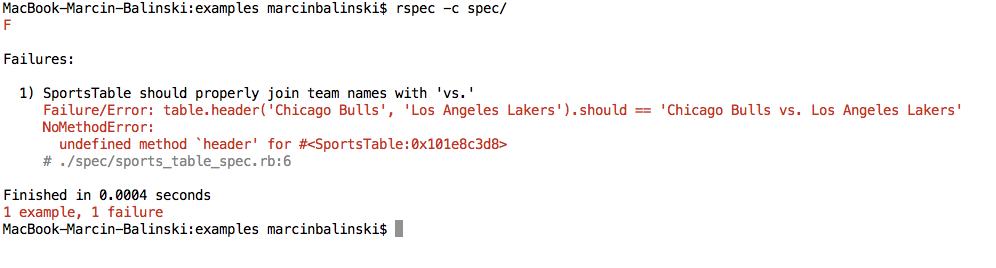
\includegraphics[width=160mm]{images/example1_failure.png}
    
    Tym samym zakończyliśmy pierwszy etap: opisaliśmy wymagane zachowanie testem oraz upewniliśmy się, że test nie przechodzi. Następnym krokiem jest napisanie pierwszej wersji metody \verb+header+:
    
    \lstinputlisting[language=ruby]{examples/code/ch02/02.rb}
    
    Ponowne uruchomienie zestawu testów kończy się sukcesem:
    
    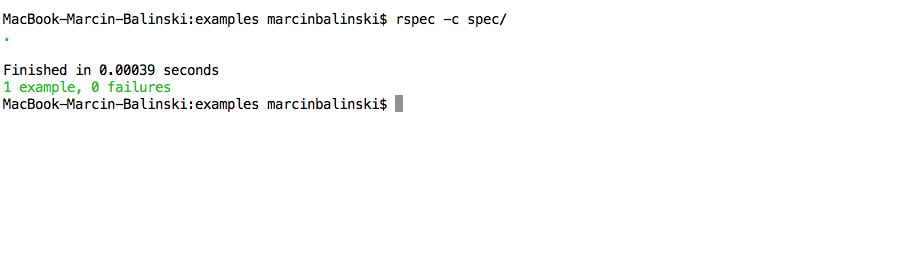
\includegraphics[width=160mm]{images/example1_success.png}
    
    Nasza metoda spełnia wszystkie założenia opisane przez testy, wciąż jednak jest pole do poprawy jakości kodu. W języku Ruby każda metoda domyślnie zwraca ostatnią zdefiniowaną w swoim ciele wartość, możemy więc zrezygnować ze zbędnego słowa kluczowego \verb+return+. Oprócz tego zmienimy sposób konstrukcji wynikowego łańcucha: zrezygnujemy z operatora \verb+++ na rzecz metody \verb+join+ obiektu klasy \verb+Array+. Po modyfikacji metoda \verb+header+ wygląda następująco:
    
    \lstinputlisting[language=ruby]{examples/code/ch02/03.rb}
    
  Powtórne uruchomienie zestawu testów kończy się sukcesem, a pierwsza iteracja TDD jest zakończona. Zdołaliśmy opisać nową funkcjonalność oraz poprawnie ją zaimplementować. W tym miejscu należy dodać, że w trzecim kroku, po modyfikacji i ulepszeniu kodu nie zmodyfikowaliśmy zestawu testów. W tym konkretnym przypadku najważniejszy dla nas jest wynik działania metody \verb+header+, nie zaś szczegóły implementacji. Nie testujemy np. tego, że konstrukcja wynikowego łańcucha znaków odbywa się z użyciem metody \verb+join+. Czasami jednak szczegóły implementacji są równie ważne jak zwracane wynik i wtedy należy napisać odpowiednie testy.
    
  \subsection{Zalety TDD}
    Test Driven Development wymusza na programiście konkretną dyscyplinę pracy. Proces rozwoju oprogramowania jest iteracyjny i bardzo uporządkowany a także wymaga uprzedniego zaplanowania każdej zmiany lub dodatku do istniejącej bazy kodu. Każda iteracja może zostać zakończona jedynie, gdy wszystkie testy zakończą się sukcesem. Taki sposób pracy niesie ze sobą wiele zalet, między innymi:
     
    \begin{itemize}
      \item Pewność, że oprogramowanie zawsze działa zgodnie z założeniami
      \item Wzrost produktywności
      \item Wzrost jakości kodu
      \item Minimalizacja liczby defektów
      \item Możliwość wczesnego wykrycia defektów
      \item Modularyzacja kodu jako pozytywny skutek uboczny
    \end{itemize}

  \section{Narzędzia wspierające TDD dostępne dla języka Ruby}
    
    \subsection[Test::Unit]{Test::Unit\footnote{\url{http://test-unit.rubyforge.org/test-unit/}\nocite{test_unit}}}
    
    Test::Unit należy do bibliotek dołączanych standardowo do każdej dystrybucji języka Ruby. Oprogramowanie testujemy tutaj przy pomocy tak zwanych asercji. Najprostsza asercja ma postać wywołania metody \verb+assert+, która sygnalizuje niepowodzenie testu w momencie, kiedy wyrażenie przekazane jako jej parametr jest fałszem, przykładowo:
    
    \lstinputlisting[language=ruby]{examples/code/ch02/04.rb}
     
     \subsubsection{Konstrukcja zestawu testów}
     Zestaw testów biblioteki Test::Unit ma postać definicji klasy, która dziedziczy po klasie Test::Unit::TestCase. Pojedyncze testy definiujemy jako metody, rozpoczynające się od ciągu znaków \emph{test}. W ciele każdej z takich metod możemy zdefiniować wiele asercji (aczkolwiek idealnie jest, jeśli jeden test równoznaczny jest z jedną asercją). Test kończy się sukcesem jedynie, kiedy wszystkie należące do niego asercję również zakończą się sukcesem.
     
     Przykładowy prosty zestaw testów opisujących zachowanie aplikacji będącej kalkulatorem może wyglądać tak:
     
     \lstinputlisting[language=ruby]{examples/code/ch02/05.rb}
     
     Oprócz metody \verb+assert+ biblioteka oferuje bardziej wyspecjalizowane typy asercji:
     
     \begin{description}
       \item[assert\_equal(expected, actual)] przyjmuje dwa parametry, zwraca prawdę, jeśli parametry są sobie równe.
       \item[assert\_not\_equal(expected, astual)] przyjmuje dwa parametry, zwraca prawdę, jeśli parametry różne od siebie.
       \item[assert\_match(regex, string)] przyjmuje dwa parametry w postaci łańcucha znaków lub wyrażenia regularnego, zwraca prawdę jeśli nastąpi dopasowanie wzorca.
       \item[assert\_no\_match(regex, string)] przyjmuje dwa parametry w postaci łańcucha znaków lub wyrażenia regularnego, zwraca prawdę jeśli dopasowanie wzorca nie nastąpi.
       \item[assert\_nil(object)] zwraca prawdę jeśli przekazany parametry ma pustą wartość (\verb+nil+).
       \item[assert\_not\_nil(object)] zwraca prawdę, jeśli przekazany parametr ma niepustą wartość (różną od \verb+nil+).
       \item[assert\_instance\_of(class, object)] przyjmuje na wejściu nazwę klasy oraz parametr, zwraca prawdę, jeśli parametr jest obiektem typu \verb+class+.
    \end{description}
    
    \subsubsection{Warunki początkowe i końcowe}
    Czasem grupa testów powinna być uruchamiana przy takich samych warunkach początkowych, albo też (nie tak częsty przypadek) występuje konieczność wykonania jakichś czynności na koniec każdego testu (np. wyczyszczenie bazy danych). Biblioteka Test::Unit pozwala definiować warunki początkowe i końcowe przy pomocy metod \verb+setup+ i \verb+teardown+.
    Metoda \verb+setup+ zostanie wykonana przed każdym testem, metoda \verb+teardown+ bezpośrednio po każdym teście. Możemy np. znacząco uprościć nasz przykładowy zestaw testów kalkulatora poprzez przeniesienie procesu tworzenia obiektu Calculator do metody setup. zmodyfikowane testy używają również bardziej właściwych asercji:
    
    \lstinputlisting[language=ruby]{examples/code/ch02/06.rb}
    
    Przedrostek \verb+@+ przy zmiennej \verb+calc+ oznacza, że odnosimy się do zmiennej instancyjnej a więc dzielonej w obrębie obiektu danej klasy, zmienne bez tego przedrostka traktowane są w Ruby jako zmienne lokalne.
    
    \subsubsection{Pakiety testów}
    Testując dużą aplikację będziemy chcieli podzielić testy na kilka plików tak, aby odzwierciedlić modułową budowę aplikacji oraz poprawić czytelność testów. Biblioteka Test::Unit upraszcza proces uruchamiania całego pakietu testów. Jedyne co musimy w tym wypadku zrobić to stworzyć nowy plik i przy pomocy metody \verb+require+ załadować wszystkie pliki zawierające interesujące nas testy:
    
    \lstinputlisting[language=ruby]{examples/code/ch02/07.rb}
    
    Teraz, jeśli wykonamy polecenie:
    
    \begin{lstlisting} 
      ruby test/full_suite.rb
    \end{lstlisting}
    
    uruchomione zostaną wszystkie testy zdefiniowane w plikach:
    
    \begin{lstlisting} 
      test/test_suite1.rb
      test/test_suite2.rb
      test/test_suite3.rb
    \end{lstlisting}
    
    \subsection[RSpec]{RSpec\footnote{\url{http://rspec.info/}\nocite{rspec}}}
    % dokładniejszy opis, trochę więcej o tym, dlaczego powstał RSPEC
    
    Kolejnym narzędziem świetnie wspierającym testowanie oprogramowania w języku Ruby jest biblioteka RSpec. RSpec jest narzędziem bardziej rozbudowanym niż Test::Unit, w tym podrozdziale skupię się jednak na jego podstawowych funkcjach umożliwiających testowanie oprogramowania w zgodzie z filozofią TDD.
    
    Bibliotekę RSpec najłatwiej zainstalować przy pomocy narzędzia ruby gems, które jest standardowo dostarczane wraz z każdą dystrybucją języka Ruby. Proces instalacji jest trywialny, wystarczy z konsoli systemowej wydać polecenie:
    
    \begin{lstlisting}
    gem install rspec
    \end{lstlisting}
    
    \subsubsection{Przykłady}
    W RSpec każdy test nazywany jest przykładem (ang. example). RSpec definiuje własny dialekt języka Ruby, dzięki czemu przykłady wyglądają bardziej jak naturalny język. W początkowej części tego rozdziału zdefiniowaliśmy już przykłady dla oprogramowania obsługującego sportową tablicę wyników:
    
    \lstinputlisting[language=ruby]{examples/code/ch02/08.rb}
    
    Pierwsze co powyższy kod robi, to dołącza plik z klasą \verb+SportsTable+, którą mamy zamiar przetestować. Zaraz później znajduje się linia:
    
    \begin{lstlisting}
    describe SportsTable do
    \end{lstlisting}
    
    Metoda \verb+describe+ zwraca tak zwaną grupę przykładów, która w bibliotece RSpec implementowana jest przez klasę \verb+ExampleGroup+. Jako parametry przyjmuje ona testowaną klasę oraz opcjonalny opis. Metoda \verb+describe+ przyjmuje też blok kodu, który programista definiuje pomiędzy słowami kluczowymi \verb+do ... end+.
    
    Konkretne przykłady zdefiniowane są w bloku przekazanym do metody \verb+describe+. Przykład definiuje metoda \verb+it+, której parametrem jest łańcuch znaku będący opisem a sam przykład zdefiniowany w przekazywanym do tej metody bloku.
    
    \subsubsection{Oczekiwania}
    Oczekiwanie jest odpowiednikiem asercji znanych z Test::Unit, w bibliotece RSpec mechanizm oczekiwań zaimplementowany jest w module Spec::Expectations w taki sposób, że do każdego obiektu dynamicznie dodawane są metody \verb+should+ oraz \verb+should_not+. Każda z tych metod jako parametr przyjmuje kolejne wyrażenie dopasowujące (ang. Matcher) wyrażenia takie można definiować samemu, albo pozwolić aby RSpec zdefiniował je dynamicznie. Przykładowe oczekiwania, które dynamicznie rozumie RSpec:
    
    \lstinputlisting[language=ruby]{examples/code/ch02/09.rb}
    
    % prościej?
    W języku Ruby metody, które kończą się znakiem zapytania w zgodzie z konwencją powinny być metodami które zwracają prawdę lub fałsz. Metoda taka testuje po prostu jakieś założenie w stosunku do obiektu danej klasy. Przykładowo metoda \verb+empty?+ obiektu klasy Array testuje czy dana tablica jest pusta zwracając wartość \verb+true+ jeśli tak jest, lub \verb+false+ w przeciwnym wypadku. Automatyczne sprawdzanie oczekiwań w bibliotece RSpec korzysta właśnie z tej konwencji w taki sposób, że jeśli nie uda się znaleźć zdefiniowanego wyrażenia dopasowującego o danej nazwie RSpec szuka metody obiektu o tej samej nazwie zakończonej dodatkowo znakiem zapytania. W tym procesie pomijane są pewne początkowe słowa kluczowe takie jak \verb+be_+, \verb+a_+ czy \verb+an_+ co pozwala to na konstruowanie przykładów tak, aby bardziej przypominały naturalny język. W powyższych przykładach do sprawdzenia prawdziwości testu kolejno wykorzystywane są następujące metody obiektu klasy Array: \verb+empty?+, \verb+include?+, \verb+instance_of?+
    
    \subsubsection{Imitacje obiektów}
    W trakcie testowania oprogramowania zdarzają się sytuacje, kiedy chcemy uniknąć korzystania z prawdziwych instancji jakiejś klasy. Najczęściej jest tak w przypadku, kiedy dany obiekt nie jest bezpośrednio przedmiotem testu, ale inna część oprogramowania polega na nim, lub jeśli wykonuje on kosztowne operacje, które spowalniają testy.
    
    RSpec pozwala w takim przypadku na definiowanie tak zwanych imitacji obiektów. Imitacja (ang. Mock) to w skrócie obiekt-atrapa, programista deklaruje na jakie komunikaty ma odpowiadać. Wyobraźmy sobie, że pewien moduł naszego systemu wykonuje bardzo czasochłonne operacje matematyczne, na wynikach tych operacji polega drugi moduł, który chcemy przetestować. W takiej sytuacji moglibyśmy oczywiście skonstruować test tak, że faktycznie inicjowalibyśmy cały proces obliczeniowy modułu matematycznego, a jego wynik przekazywali do testowanego modułu jednak taka metoda szybko sprawiłaby, że nasze testy byłyby bardzo powolne. 
    
    Jeśli moduł matematyczny sam w sobie jest dobrze przetestowany, to nic nie stoi na przeszkodzie, aby przy testowaniu zależnej od niego części systemu użyć już tylko jego imitacji. W Rspec może to wyglądać w taki sposób:
    
    \lstinputlisting[language=ruby]{examples/code/ch02/10.rb}
    
    Zakładamy tutaj, że metoda \verb+run+ obiektu klasy \verb+CoolPartUsingMathsModule+ korzysta z wyniku jaki zwraca metoda \verb+compute+ obiektu typu \verb+MathsModule+. Metoda \verb+mock+ zwraca imitacje obiektu. Klasę obiektu definiujemy jako pierwszy argument, następnie występuje opcjonalna lista komunikatów wraz ze zwracaną wartością, na te komunikaty atrapa będzie odpowiadać.
    
    Test ten można skonstruować jeszcze lepiej. W aktualnej formie nie stawiamy w nim bowiem żadnych warunków jakie musi spełniać testowana metoda \verb+run+. Zdefiniowaliśmy w prawdzie imitację obiektu matematycznego, która odpowiada na wywołanie metody \verb+compute+ zwracając wartość \verb+1337+, nie sprawdzamy jednak, czy metoda ta kiedykolwiek zostaje wykonana. Chcąc upewnić się, że tak faktycznie jest możemy napisać powyższy test tak:
    
    \lstinputlisting[language=ruby]{examples/code/ch02/11.rb}

    
    Wywołując na obiekcie metodę \verb+should_receive+ definiujemy nowe oczekiwanie: teraz test zakończy się sukcesem tylko wtedy, kiedy nastąpi dokładnie jedno wywołanie metody \verb+compute+. W taki sposób przetestowaliśmy integrację pomiędzy naszymi modułami i jednocześnie sprawiliśmy, że test jest bardzo szybki, nie wykonuje on bowiem żadnych obliczeń modułu matematycznego, a zamiast tego korzysta z bardzo prostej atrapy.
	\chapter[Behavior Driven Development]{Behavior Driven Development}
  \section{Czym jest BDD?}
    Behavior Driven Development jest metodyką rozwoju oprogramowania, w której główny nacisk położony jest na zacieśnienie współpracy między programistami, a nietechnicznymi uczestnikami projektu. Podobnie jak w przypadku TDD implementację konkretnej funkcjonalności poprzedza zdefiniowanie jej zachowania w teście. Różnica polega na tym, że scenariusze BDD pisane są w naturalnym języku, tak aby były zrozumiałe nie tylko dla programistów. Idealną sytuacją jest kiedy scenariusze takie powstają w wyniku ścisłej współpracy programistów oraz właścicieli projektu ponieważ, jak sama nazwa wskazuje, BDD kładzie nacisk na zdefiniowanie i zrozumienie zachowania aplikacji a szczegóły implementacji są tutaj mniej istotne.
    \subsection{BDD jako narzędzie dokumentacji. Funkcjonalności i scenariusze}
      Każdy program tak naprawdę składa się z zestawu funkcjonalności. Każda funkcjonalność wnosi konkretną wartość dodaną z punktu widzenia grupy docelowej, dla której oprogramowanie powstaje. Przykładowo program do obsługi księgowości powinien pozwalać zarządzać rachunkiem zysków i strat oraz sporządzać bilans (to oczywiście tylko niektóre z funkcji). Każda wyżej wymienionych czynności to pojedyncza funkcjonalność, która w zgodzie z filozofią BDD powinna zostać opisana zestawem scenariuszy.
      
      Scenariusze opisują zachowanie się programu w kontekście konkretnej funkcjonalności w precyzyjnie zdefiniowanej sytuacji a dla każdej funkcjonalności możemy zdefiniować dowolną ilość scenariuszy użycia. Na przykład dla funkcjonalności Zarządzanie rachunkiem zysków i strat mogą być zdefiniowane następujące scenariusze:
      
      \begin{itemize}
        \item Wprowadzenie nowej poprawnej pozycji
        \item Wprowadzenie nowej nie poprawnej pozycji
        \item Modyfikacja pozycji
        \item Próba wprowadzenia nowej pozycji przez nieautoryzowanego użytkownika
      \end{itemize}
      
      Narzędzia BDD pozwalają na bardzo dużą swobodę jeśli chodzi o język definiowania scenariuszy, przykładowy plik definiujący powyższą funkcjonalność wraz ze scenariuszem 'Wprowadzenie nowej nie poprawnej pozycji' mógłby wyglądać tak:
      
\begin{verbatim}
  Funkcjonalność: Zarządzanie rachunkiem zysków i strat
  
  Scenariusz: Wprowadzenie nowej nie poprawnej pozycji
    Jako zalogowany użytkownik systemu
    Kiedy wybieram z menu głównego pozycję "Wprowadź nową pozycję"
    Oraz wprowadzam do pola "Przychody netto ze sprzedaży produktów" wartość "to_nie_jest_liczba"
    Wtedy powinienem zobaczyć wiadomość "Błąd: Niepoprawna wartość. To pole jest polem liczbowym."
    Oraz pole "Przychody netto ze sprzedaży produktów" powinno być puste
\end{verbatim}

    Powyższy przykład opisuje zachowanie aplikacji w sposób na tyle naturalny, że nikt nie będzie miał trudności w jego zrozumieniu, a po poznaniu kilku prostych zasad językowych, którymi należy się kierować również nie techniczny uczestnicy projektu mogą opisywać nowe funkcjonalności w ten sposób.
    
    Tworzenie specyfikacji projektu w postaci scenariuszy BDD jest bardzo pożądane. Zmniejsza to ilość niepotrzebnej dokumentacji, powoduje zacieśnienie współpracy w zespole oraz, o czym więcej w następnym podrozdziale, zwiększa pokrycie kodu testami.
    
    \subsection{BDD jako narzędzie testowania}
      Prawdziwą mocą bibliotek wspierających Behavior Driven Development jest to, że traktują one specyfikacje dostarczoną w postaci scenariuszy jako zestaw testów. Dołączając więc scenariusze do naszego zestawu testów automatycznych mamy pewność, że oprogramowanie zachowuje się zgodnie z opisanymi w nich założeniami. W tym podrozdziale chciałbym opisać w jaki sposób, z technicznego punktu widzenia przebiega proces translacji specyfikacji (będącej plikiem tekstowym składającym się z pojedynczych scenariuszy) na zestaw automatycznych testów.
      \subsubsection{Definicje kroków na przykładzie biblioteki Cucumber}
        Aby skutecznie uruchomić scenariusze w formie testów należy skonstruować plik tekstowy je zawierający w zgodzie z pewnymi zasadami. Przykładowy plik definiujący funkcjonalność 'Zarządzanie rachunkiem zysków i strat' rządzi się pewnymi prawami:
        
        \begin{itemize}
          \item Nazwa opisywanej funkcjonalności zdefiniowana jest po słowie kluczowym 'Funkcjonalność:'
          \item Pojedyncze scenariusze definiowane są po słowie kluczowym 'Scenariusz:'. Należą do ostatnio zdefiniowanej funkcjonalności.
          \item Każda kolejna linia nie będąca definicją nowego scenariusza lub funkcjonalności traktowana jest jako pojedynczy krok ostatnio zdefiniowanego scenariusza.
        \end{itemize}
        
      Sercem biblioteki Cucumber są definicje kroków, które pozwalają powiązać każdy z nich z konkretną akcją. Definicja kroku składa się z wzorca językowego kroku oraz kodu który ma zostać wykonany jeśli wzorzec pasuje do aktualnie przetwarzanego kroku.
      
      Wzorzec językowy najczęściej przybiera postać wyrażenia regularnego. Cucumber przetwarzając nowy krok iteruje po wzorcach, które zostały zdefiniowane i wykonuje kod powiązany z pierwszym, do którego pasuje nazwa kroku (dlatego ważne jest definiowanie wzorców tak, aby były unikalne). Przykładowa definicja dla kroku 'Kiedy wybieram z menu głównego pozycję "Wprowadź nową pozycję"' może wyglądać tak:
      
      \begin{verbatim}
        Kiedy /wybieram z menu głównego pozycję "(.*)"/ do |pozycja|
          # zmienna 'pozycja' zawiera teraz ciąg znaków, który dopasowany został
          # do wyrażenia "(.*)" a więc dla kroku 'Kiedy wybieram z menu głównego pozycję "Wprowadź nową pozycję"'
          # będzie miała wartość: Wprowadź nową pozycję
        end
      \end{verbatim}
      
      Kiedy cucumber spróbuje przetworzyć krok 'Kiedy wybieram z menu głównego pozycję "Wprowadź nową pozycję"' dopasuje go do pierwszego odpowiadającego wzorca, który zdefiniowaliśmy oraz uruchomi blok kodu zdefiniowany pomiędzy słowami kluczowymi \verb+do+ oraz \verb+end+. Przekaże do tego bloku również wszelkie zmienne zdefiniowane we wzorcu. Powyższy przykład jest na razie bezużyteczny ponieważ jedyne co znajduje się w bloku kodu to komentarz.
      
      Krok scenariusza najczęściej definiuje jedną z trzech rzeczy: założenie co do stanu środowiska w jakim uruchomione jest oprogramowanie, konkretną akcję wykonywaną na oprogramowaniu (taką jak np. kliknięcie przycisku) lub rezultat, jakiego się spodziewamy. Cucumber sam w sobie jest narzędziem które dopasowuje krok do odpowiadającej mu definicji, wszelkie interakcje z działającym programem, modyfikowanie środowiska działania czy też testowanie otrzymywanych wyników muszą zostać wykonywane przez zewnętrzne biblioteki, które należy samodzielnie skonfigurować.
      
      Aby lepiej zobrazować w jaki sposób może wyglądać działające środowisko BDD poczynię kilka założeń co do aplikacji, którą testujemy, oraz bibliotek, których użyjemy. Pominę szczegóły konfiguracji, jest to treścią jednego z kolejnych rozdziałów tej pracy.
      
      \begin{itemize}
        \item Interfejs naszej aplikacji zdefiniowany jest językiem opisu dokumentów HTML.
        \item Aplikacja napisana jest w języku Ruby, przy pomocy frameworka Ruby on Rails
        \item Narzędzie RSpec zostało zainstalowane i skonfigurowane
        \item Narzędzie Capybara zostało zainstalowane i skonfigurowane
      \end{itemize}
      
      O bibliotece RSpec pisałem już w poprzednim rozdziale, tutaj użyjemy go w podobnym celu, to jest do testowania wyników działania aplikacji. Biblioteka Capybara służy do symulacji interakcji użytkownika z aplikacją używającą jako interfejsu HTML. Używając powyższych narzędzi mogę opisać pełen zestaw definicji kroków dla scenariusza 'Wprowadzenie nowej nie poprawnej pozycji':
      
      \begin{verbatim}        
        Jako /zalogowany użytkownik systemu/ do
          # znajdź pierwszego zarejestrowanego użytkownika
          user = User.first
          # otwórz stronę logowania
          visit "/login"
          # wypełnik pola 'email' i 'hasło' poprawnymi danymi
          fill_in("email", :with => user.email)
          fill_in("hasło", :with => user.password)
          click_button("Zaloguj")
        end
        
        Kiedy /wybieram z menu głównego pozycję "(.*)"/ do |pozycja|
          select(pozycja, :from => "menu główne")
        end
        
        Oraz /wprowadzam do pola "(.*)" wartość "(.*)"/ do |pole, wartosc|
          fill_in(pole, :with => wartosc)
        end
        
        Wtedy /powinienem zobaczyć wiadomość "(.*)"/ do |wiadomosc|
          response.should contain(wiadomosc)
        end
        
        Oraz /pole "Przychody netto ze sprzedaży produktów" powinno być puste/ do |pole|
          field_labeled(pole).value.should be_empty
        end
      \end{verbatim}
      
    \subsubsection{Rola programisty}
    
      Jak widać definiowanie kroków wymaga podstawowej wiedzy z zakresu programowania oraz budowy opisywanego systemu, dlatego też zadanie to najczęściej wykonują programiści pracujący nad projektem.  Klient w tym wypadku dostarcza specyfikacji w postaci scenariuszy użycia, programiści zaś definiują brakujące kroki. Na szczęście problem ten jest uciążliwy właściwie tylko na początku życia projektu. Wraz z rosnącą ilością scenariuszy rośnie też ilość definicji kroków, a w pewnym momencie życia projektu definicje kroków zaczynają gęsto pokrywać większość funkcjonalności systemu tak, że w większości wypadków nawet do nowych funkcjonalności można bez problemu dopasować istniejące już kroki.
      
      Ważne jest aby scenariusze były jak najbardziej zestandaryzowane, to znaczy, aby w miarę możliwości korzystać z już zdefiniowanych kroków w procesie ich tworzenia. Aby to osiągnąć osoba odpowiedzialna  za dostarczenie specyfikacji w postaci scenariuszy powinna poświęcić trochę czasu na zapoznanie się z dostępnymi definicjami kroków.
      
      Ze strony programistów, którzy piszą definicje szczególny nacisk powinien zostać położony na kilka kwestii:
      
      \begin{description}
        \item[Unikanie powtórzeń] Należy upewnić się, że brakujący krok jest na pewno unikalny. Może okazać się, że wcześniej został zdefiniowany bardzo podobny krok, o innej nazwie.
        \item[Parametryzacja] Jeśli zachodzi taka potrzeba należy przystosować definicję kroku tak, aby obsługiwała więcej niż jeden przypadek użycia.
        \item[Klasyfikacja] Aby zwiększyć czytelność kodu należy klasyfikować kroki na przykład według funkcjonalności, które obsługują, można w tym celu umieszczać kroki w osobnych plikach.
      \end{description}
      
      Przestrzeganie tych zasad nie jest konieczne do poprawnego działania systemu ale na pewno w znaczącym stopniu poprawi czytelność i jakość naszej bazy testów.
      
    \subsection{Testy akceptacyjne a BDD}
      
      Kiedy nowa funkcjonalność jest skończona klient zawsze powinien ją przetestować i zaakceptować jeśli spełnia jego oczekiwania, lub odrzucić w przeciwnym wypadku. W tradycyjnym podejściu do rozwoju oprogramowania testy akceptacyjne wyglądają najczęściej tak, że klient ręcznie sprawdza nową funkcjonalność. Minusy manualnego testowania zostały szczegółowo opisane w rozdziale dotyczącym TDD. Behavior Driven Development pozwala w dużym stopniu wyeliminować czasochłonne manualne testy akceptacyjne. W momencie, kiedy mamy gotowy dobry zestaw scenariuszy użycia, który jednocześnie jest specyfikacją funkcjonalności sam fakt, że wszystkie scenariusze zostają uruchomione z pozytywnym skutkiem jest wystarczającym testem akceptacyjnym.
      
      Jeśli chcemy zastąpić testy akceptacyjne z żywym klientem na scenariusze BDD należy pamiętać, że środowisko testowe (w tym definicje kroków) muszą zostać zaprojektowane tak, aby działały w identycznej konfiguracji jak konfiguracja produkcyjna (czyli taka, w jakiej działa nasze oprogramowanie po dostarczeniu do klienta). Szczególnie nie należy używać imitacji (ang. mock) obiektów, których bardzo często używa się w testach jednostkowych, scenariusze powinny testować zachowanie się aplikacji w naturalnym środowisku.
      
  \section{Narzędzia BDD dostępne dla języka Ruby}
    \subsection{Cucumber}
      W środowisku programistów języka Ruby najpopularniejszym narzędziem BDD jest bez wątpienia biblioteka Cucumber. Cucumber powstał w 2008 roku jako następca biblioteki Story Runner będącej częścią narzędzia RSpec. Biblioteka miała umożliwić programistom opisywanie naturalnym językiem sposobu w jaki powinno zachowywać się oprogramowanie. Scenariusze służą jednocześnie jako dokumentacja oraz zestaw automatycznych testów. 
      
      Niewątpliwą zaletą biblioteki Cucumber jest to, że możne ona współpracować również z innymi niż Ruby platformami programistycznymi takimi jak Java, .NET, Adobe Flex czy Python. Więcej informacji na ten temat znaleźć można pod adresem: http://github.com/aslakhellesoy/cucumber/wiki.
      
      Instalacja jest równie prosta jak w przypadku omawianej wcześniej biblioteki RSpec:
      
      \begin{verbatim}
        gem install cucumber
      \end{verbatim}
      
      Jako, że techniki prezentowane w tym rozdziale opisane i zaprezentowane zostały na przykładzie biblioteki Cucumber powtórny szczegółowy opis tego narzędzia jest w tym miejscu zbędny. Szczegółowa dokumentacja dostępna jest pod adresem: http://cukes.info
      
    \subsection{Steak}
      Steak podobnie jak Cucumber jest narzędziem, które służy do opisywania zachowania aplikacji w formie automatycznych testów, główny nacisk jest tutaj jednak kładziony na wygodę programisty oraz szybkość powstawania testów. Ograniczenia w stosunku do tego co oferuje Cucumber są następujące:
      
      \begin{itemize}
        \item Brak wsparcia dla naturalnego języka
        \item Brak podziału na scenariusze oraz kroki
        \item Konieczność pisania testów w Ruby
      \end{itemize}
      
      Steak rezygnuje z filozofii angażowania nie technicznych uczestników projektu w cykl testowania oprogramowania wychodząc z założenia, że opcja ta i tak nie jest wykorzystywana w większości projektów informatycznych. Programista sam konstruuje testy w języku Ruby, nie jest to tak czytelne jak w przypadku Cucumbera, jednak ich tworzenie i utrzymanie jest prostsze:
      
      \begin{itemize}
        \item Definicje kroków są zbędne
        \item Nie trzeba ustalać i trzymać się konwencji językowych
        \item Bezpośredni dostęp do wszystkich funkcji języka Ruby
      \end{itemize}
      
      Przykładowa specyfikacja napisana przy pomocy biblioteki Steak wygląda następująco:
      
      \begin{verbatim}
      feature "Main page" do

          background do
            create_user :login => "jdoe"
            login_as "jdoe"
          end

          scenario "should show existing quotes" do
            create_quote :text => "The language of friendship is not words, but meanings",
                         :author => "Henry David Thoreau"

            visit "/"

            page.should have_css(".quote", :count => 1)
            within(:css, ".quote") do
              page.should have_css(".text", :text => "The language of friendship is not words, but meanings")
              page.should have_css(".author", :text => "Henry David Thoreau")
            end
          end

        end
      \end{verbatim}
      
      Instalacja jak zwykle w przypadku (ogromnej większości) bibliotek Ruby sprowadza się do
      
      \begin{verbatim}
        gem install steak
      \end{verbatim}
      
      W przypadku, kiedy nasza aplikacja oparta jest o framework Rails, Steak oferuje dodatkowe udogodnienia, ale wymaga również minimalnie więcej konfiguracji. Wszelkie kroki są jasno opisane pod adresem http://github.com/cavalle/steak
      
      Steak jest dobrym rozwiązaniem jeśli projekt prowadzony jest przez stricte techniczny zespół lub zarząd projektu nie jest przekonany do uczestniczenia w procesie specyfikowania oprogramowania w formie testów. Minusem rezygnacji z takiej formy współpracy jest niestety spadek znaczenia tworzonej w Steaku specyfikacji jako testów akceptacyjnych: jeśli właściciele projektu nie będą rozumieli specyfikacji w formie jaką oferuje to najprawdopodobniej testy akceptacyjne będą chcieli przeprowadzić osobiście.
    
    \subsection{Capybara}  

      Capybara ułatwia integracyjne testowanie aplikacji działających w przeglądarce www symulując akcję jakie wykonywałby żywy użytkownik. Nie jest to narzędzie związane stricte z BDD, jednak świetnie uzupełnia i wspomaga biblioteki takie jak Cucumber czy Steak.
      
      Chcąc opisać krok po kroku zachowanie aplikacji internetowej, naturalnym jest łączenie akcji, które wykonuje w przeglądarce użytkownik z ich konsekwencjami. Przykładowo w celu zalogowania się należy najpierw wypełnić pole tekstowe 'Login', następnie wpisać hasło do pola 'Hasło' oraz ostatecznie kliknąć przycisk 'Zaloguj'. Capybara pozwala symulować interakcje użytkownika z naszą aplikacją w przeglądarce i wykonywać na niej takie akcje jak kliknięcie w link, wypełnienie pola czy odświeżenie strony.
      Informacją zwrotną, która często służy do określenia efektu naszych działań jest obiekt \verb+page+, który przechowuje ostatnią wyświetloną użytkownikowi stronę. Przykładowo kod:
      
      \begin{verbatim}
        feature "signing up" do
          background do
            User.create(:email => 'user@example.com', :password => 'caplin')
          end

          scenario "signing in with correct credentials" do
            within("#session") do
              fill_in 'Login', :with => 'user@example.com'
              fill_in 'Password', :with => 'caplin'
            end
              click_link 'Sign in'
              assert_true page.has_content?('Successfuly logged in!')
            end
          end
        end
      \end{verbatim}
      
      Wypełni wszelkie konieczne do zalogowania się pola, zasymuluje kliknięcie przycisku z etykietą 'Sign in' oraz sprawdzi, czy w wyniku tego, na nowo wyświetlonej stronie znajduje się treść 'Successfuly logged in!'.
      
      Instalacja podstawowej biblioteki odbywa się poprzez:
      
      \begin{verbatim}
        gem install capybara
      \end{verbatim}
      
      Tak jak w przypadku Cucumbera, funkcje Capybary wykorzystywane były w tym rozdziale w celu zobrazowania założeń BDD. Dokładna dokumentacja bardzo bogatych możliwości biblioteki wykracza poza ramy tej pracy, można ją jednak odnaleźć wraz ze szczegółami konfiguracji dla różnych środowisk na stronie http://github.com/jnicklas/capybara.
      
	% Copyright 2011, Marcin Baliński

\chapter[Studium przypadku: Dynamicznie generowany panel administracyjny]{Studium przypadku: Dynamicznie generowany panel administracyjny}
  \section{Wstęp}
  Świat technologii informatycznych zmienia się bardzo szybko. Ogromnemu skokowi mocy obliczeniowej sprzętu komputerowego towarzyszył w ostatnich kilku latach znaczący spadek cen związanych z jego wykorzystaniem. Stało się to katalizatorem rozwoju nowych trendów między innymi w dziedzinie wytwarzania oprogramowania. Gwałtowny wzrost zainteresowania dynamicznymi językami programowania takimi jak Ruby, Python czy JavaScript oraz pojawienie się nowych metodyk rozwoju produktów informatycznych, które coraz częściej ujmują ten proces bardziej z filozoficznego aniżeli technicznego lub biznesowego punktu widzenia jest bez wątpienia jednym z owoców tego procesu.
  
  Spadek kosztów mocy obliczeniowej skutecznie rozwiązał problem wyboru technologii realizacji projektu informatycznego: wydajność narzędzi, których użyjemy do realizacji celu stała się w większości przypadków pomijalnym lub przynajmniej drugorzędnym problemem. Dziś najważniejszym kryterium wyboru jest stopień dopasowania możliwości oraz charakterystyki rozważanej technologii do potrzeb zespołu odpowiedzialnego za rozwój projektu. Oczywiście istnieją również skrajne przypadki, w których to oprogramowanie, z różnych przyczyn, musi zostać napisane w konkretnej technologii. Te smutne przypadki stanowią jednak kroplę w morzu wykraczającą daleko poza ramy niniejszej pracy.
  
  W czasach, kiedy o wiele bardziej opłaca się dokupić nowy serwer niż pokrywać koszty optymalizacji ogromną furorę robi termin \"Przedwczesna optymalizacja\". Te dwa słowa mają dzisiaj znaczenie negatywne, które jest jednak jak najbardziej uzasadnione z ekonomicznego oraz użytkowego punktu widzenia. Dopóki niedostatki w wydajności oprogramowania można skompensować inwestycją w nowe zasoby sprzętowe zespół programistów powinien skupiać wszystkie swoje wysiłki na rozwój funkcjonalności. Optymalizacja kodu następuje dopiero w momencie, kiedy koszty inwestycji w sprzęt przewyższają koszt związane z optymalizacją albo w momencie kiedy oprogramowanie ze względu na swoją nie optymalność przestaje się skalować na nowe zasoby sprzętowe.
  
  Na pierwszy rzut oka może wydawać się, że ten wstęp niewiele ma wspólnego z tematem pracy. Należy jednak uświadomić sobie, że to właśnie opisane powyżej zmiany w sposobie myślenia o metodach prowadzenia projektów IT stoją u podstaw rozwoju nowoczesnych narzędzi takich jak wymienione wcześniej dynamiczne języki, wysokopoziomowe frameworki programistyczne na nich oparte czy metodologie pokroju Behaviour Driven Development. Środki, które służą osiągnięciu założonego celu są jedną z najważniejszych zmiennych od których zależy sukces projektu, w przeszłości istniało wiele barier ograniczających ich wybór, dziś większość z nich została usunięta.
  
  \section{Założenia projektu}
  Celem niniejszego rozdziału jest pokazanie czytelnikowi w jaki sposób rozwija się konkretny projekt prowadzony w zgodzie z metodologią BDD oraz jakie płyną z tego korzyści. Wybrany temat projektu to dynamiczny panel administracyjny dla aplikacji internetowych opartych na bibliotece Ruby on Rails, jego główne założenia to:
  
  \begin{description}
    \item[Uniwersalność] Panel powinien współpracować z większością aplikacji napisanych w Ruby on Rails. W praktyce oznacza to, że jeśli modele biznesowe powinny być klasami pochodnymi klasy \verb+ActiveRecord+ a sposób budowy aplikacji jest zgodny z konwencjami przyjętymi dla aplikacji Ruby on Rails.
    \item[CRUD] W teorii baz danych istnieją cztery podstawowe operacje jakie możemy wykonać na zasobie: Tworzenie, odczytanie, aktualizacja, usunięcie (ang. Create, read, update and delete). Biblioteka ma pozwalać na zarządzanie modelami biznesowymi aplikacji przy użyciu jedynie tych czterech standardowych metod.
    \item[Dynamiczność] Po instalacji panel powinien sam wykryć rodzaje zasobów na jakich operuje aplikacja oraz wygenerować odpowiednie widoki i formularze do zarządzania nimi. Zmiany w budowie modeli biznesowych, które wymuszają konieczność zmian w zarządzaniu nimi, jak również pojawienie się nowych modeli również powinno być odzwierciedlone w zachowaniu panelu automatycznie, bez konieczności jakiejkolwiek ingerencji.
    \item[Proste wdrożenie] Podstawowe wdrożenie rozwiązania wymaga jedynie aby aplikacja kliencka korzystała z biblioteki Ruby on Rails w wersji co najmniej 3.0.3. Po dodaniu biblioteki panelu do listy gemów wykorzystywanych przez aplikację możliwe jest natychmiastowe korzystanie.
    \item[Wygoda użytkowania] Proces zarządzania aplikacją powinien być jak najwygodniejszy. Oznacza to między innymi, że pola formularzy służących do tworzenia lub edycji rekordów powinny być dostosowane do rodzaju danych jakie przechowują a próby wprowadzenia nieprawidłowych wartości powinny być sygnalizowane czytelną informacją o błędzie. Jeśli istnieją powiązania pomiędzy kilkoma modelami biznesowymi, to powinna istnieć bardzo szybka możliwość zarządzania każdym z powiązanych rekordów.
  \end{description}
  
  \subsection{Open Source}
    Biblioteka jest dostępna za darmo na zasadach licencji MIT.\footnote{http://en.wikipedia.org/wiki/MIT\_License} Filozofia rozwoju oprogramowania na zasadach open source jest bardzo bliska środowisku programistów Ruby. Sam język udostępniony jest na licencji GPL, biblioteka Ruby on Rails korzysta z licencji MIT. Użycie licencji MIT oznacza, że każdy otrzymuje prawo do nielimitowanego wykorzystania kopii oprogramowania w dowolny sposób, sprawia to, że jest to najchętniej wykorzystywana przez programistów Ruby licencja.
    
  \subsection{Sposób prowadzenia projektu}
  Projekt prowadzony jest według bardzo uproszczonych zasad metodologii SCRUM.\footnote{http://en.wikipedia.org/wiki/Scrum\_(development)} \nocite{wiki_scrum} Rozwój projektu podzielony jest na tygodniowe sprinty, przed każdym z nich następuje spotkanie zespołu, podczas którego wybierane i przydzielane są konkretne zadania do wykonania w następnej iteracji. Spotkania te służą również omówieniu bieżących spraw związanych z projektem.
  
  Zespół zaangażowany w projekt składa się z trzech osób: dwóch programistów, oraz osoby dzielącej rolę Scrum Mastera, który odpowiedzialny jest za przygotowanie i prowadzenie spotkań oraz Product Ownera, który reprezentuje oczekiwania końcowego użytkownika dotyczące kwestii funkcjonalności oraz ekonomicznych kwestii związanych z rozwojem projektu.
  
  Duży nacisk kładziony jest na testowanie oprogramowania, testy akceptacyjne istnieją w formie zautomatyzowanych scenariuszy BDD. Każda funkcjonalność lub modyfikacja oprogramowania akceptowana jest jedynie jeśli dostarczona jest wraz z pełnym zestawem testów ją dokumentujących.
  
  \subsection{Dodatkowe narzędzia}
  Repozytorium projektu zarządzane jest przez system kontroli wersji GIT\footnote{http://git\-scm.com} a hostowane jest przez serwis GitHub.\footnote{http://github.com} Źródła projektu dostępne są publicznie pod adresem https://github.com/piotrj/administer.
  
  Jako narzędzie wspomagające proces zarządzania projektem użyta została darmowa wersja Pivotal Tracker\footnote{http://www.pivotaltracker.com}, który został zaprojektowany aby wspomagać zarządzanie projektem prowadzonym według zasad SCRUM.
  
  % może inna nazwa?
  \section{Proces implementacji}
  
  Jak zostało to wspomniane wcześniej implementacja podzielona jest na tygodniowe iteracje zwane również sprintami. Każda planowana funkcjonalność zanim zostanie zaimplementowana i stanie się częścią projektu musi zostać krytycznie oceniona pod względem użyteczności oraz opisana w formie krótkiej specyfikacji.
  
  W wypadku kiedy mamy do czynienia z rozbudowaną funkcjonalnością należy podzielić jej implementację na jak najmniejsze, spójne kawałki a każdy z tych fragmentów powinien zostać jasno opisany. Idealnie jest, kiedy fragmenty danej funkcjonalności są od siebie niezależne, to znaczy, jeśli nad każdym z nich można pracować osobno w tym samym czasie. Taka sytuacja niestety zdarza się rzadko. Jeśli dany fragment zależy od innych, należy załączyć taką informację w jego opisie.
  
  Każde nowe zachowanie opisane jest testem w postaci odpowiedniego scenariusza Cucumber. Jest to warunek konieczny, scenariusze powstają przed rozpoczęciem procesu właściwej implementacji, po zaakceptowaniu przez Product Ownera pełnią one rolę testów akceptacyjnych. Testy jednostkowe w postaci specyfikacji RSpec powstają dla części systemu, których szczegóły implementacji są istotne dla prawidłowego jego działania.
  
  \subsection{Aplikacja testowa}
  Specyfika projektu dynamicznego panelu administracyjnego utrudnia nieco pisanie scenariuszy jego użycia. Myśląc o panelu administracyjnym nigdy nie myślimy o nim jako o odrębnym bycie, jest raczej nieodłącznie związany z aplikacją, którą administruje. Aby proces testowania i specyfikowania systemu był jak najbardziej naturalny biblioteka administer rozwijana jest wraz z małą aplikacją testową.
  
  Prosty system blogowy został stworzony, aby opisać i przetestować zachowanie właściwego oprogramowania. Jedynym celem istnienia aplikacji blogowej jest przetestowanie integracji biblioteki administer z zewnętrzną aplikacją. Z technicznego punktu widzenia wszystkie testy behawioralne opisują zachowanie aplikacji testowej, która dołącza bibliotekę administer do puli wykorzystywanych przez siebie gemów. W przypadku oprogramowania, które działa na zasadzie integracji z zewnętrznym systemem taka konfiguracja środowiska testowego jest najlepsza, odpowiada bowiem faktycznemu scenariuszowi użycia. Sam blog jest niezwykle prostą aplikacją, w założeniach ma pozwalać na:
  
  \begin{itemize}
    \item Wyświetlanie artykułów
    \item Tworzenie artykułów
    \item Edycję artykułów
    \item Usuwanie artykułów
    \item Kategoryzację artykułów
    \item Tworzenie kategorii
    \item Edycję kategorii
    \item Usuwanie kategorii
  \end{itemize}
  
  % PRZEREDAGOWAĆ
  Blog świetnie nadaje się do testowania biblioteki typu administer - wszystkie powyższe funkcje, prócz pierwszej, są tak naprawdę funkcjami, które wykonywać ma panel administracyjny. W kontekście tego przykładu cel biblioteki administer jest jasny: Twórca bloga ze swojej strony musi jedynie dołączyć gem administer do projektu, zdefiniować modele biznesowe typu Post czy Kategoria, oraz dopisać akcję odpowiedzialną za wyświetlanie artykułów, cała część odpowiedzialna za akcję zarządzania modelami ma być dynamicznie wykonywana przez gem administer. 
  
  Ilustracja \ref{blog_view} przedstawia stronę z listą artykułów, jest to widok pochodzący z aplikacji testowej. Ilustracja \ref{administer_edit} przedstawia widok edycji rekordu konkretnego artykułu, funkcja ta implementowana jest przez bibliotekę administer.
  
  \begin{figure}[!h]
		\begin{center}
			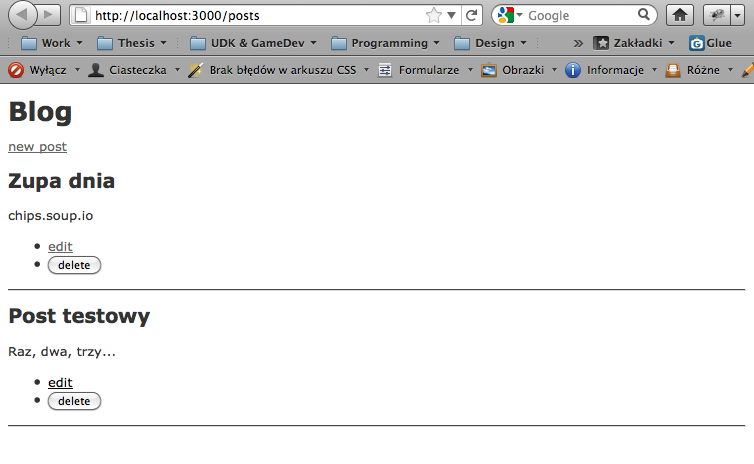
\includegraphics[width=\linewidth]{images/blog.png}
			\caption{Aplikacja testowa - wyświetlanie artykułów}
			\label{blog_view}
		\end{center}
	\end{figure}
	
	\clearpage
	
	\begin{figure}[!h]
		\begin{center}
			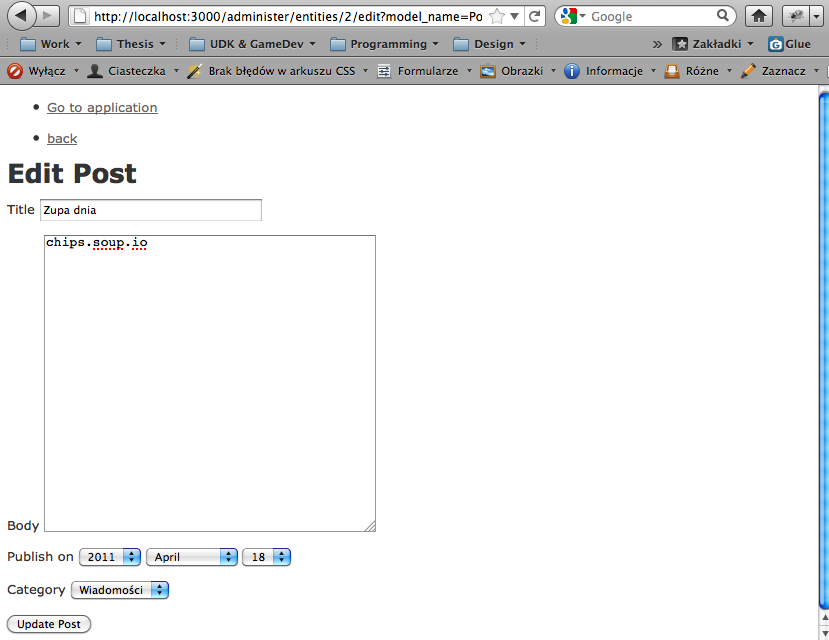
\includegraphics[width=\linewidth]{images/administer_edit.png}
			\caption{administer - edycja rekordu}
			\label{administer_edit}
		\end{center}
	\end{figure}
  
  % lepsza nazwa
  \subsection{Konfiguracja zależności testowych}
    % aplikacja testowa powinna kożystać ze źródeł testowanego gema, nie z jego release
    % Test dependencies - warto coś o tym napisać?
    
  % zdecydowanie zmień nazwę tej sekcji 
  \subsection{Implementacja funkcji usuwania rekordu}
    % screen z listą tiketów
    % dokładny opis całego procesu + wycinki kodu źródłowego dla konkretnego tiketa
    
    Ilustracja \ref{administer_stories}  przedstawia wycinek listy zadań związanych z pracą nad projektem administer a konkretnie są to zadania związane z rozwojem panelu administracyjnego.
    
    \clearpage
    
    \begin{figure}
  		\begin{center}
  			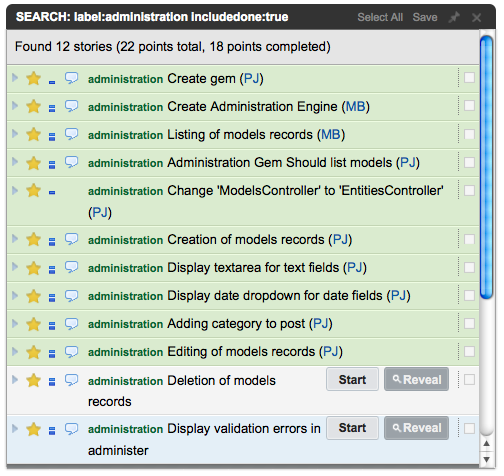
\includegraphics[width=\linewidth]{images/administer_stories_list.png}
  			\caption{Lista zadań do wykonania}
  			\label{administer_stories}
  		\end{center}
  	\end{figure}
  	
    Jako, że projekt jest rozwijany już od jakiegoś czasu, większość zadań z tej listy jest już wykonana, znajdziemy jednak dwa nadal nie rozwiązane problemy:
    
    \begin{itemize}
      \item Deletion of model records
      \item Display validation errors in administer
    \end{itemize}
    
    Skupmy się na rozwiązaniu pierwszego z nich. W momencie pisania tego rozdziału gem administer potrafi już tworzyć, modyfikować oraz wyświetlać informacje o rekordach modeli biznesowych aplikacji, która z niego korzysta. Jedną z brakujących funkcji jest usuwanie istniejących rekordów. W tym podrozdziale przeanalizujemy krok po kroku cały cykl wdrażania tej nowej funkcji do istniejącego systemu. Przeanalizowanie tego procesu pomoże nam lepiej zrozumieć sposób w jaki rozwijane jest oprogramowanie w zgodzie z zasadami BDD oraz korzyści z tego płynące.
    
    \subsubsection{Zrozumienie problemu}
    Pierwszy etap pracy to rozpoznanie, z czym tak właściwie mamy do czynienia. Jeśli problem, który mamy rozwiązać został wcześniej udokumentowany, tak jak miało to miejsce w tym wypadku, należy zacząć od dokładnego zaznajomienia się z jego opisem.
    
    Ilustracja \ref{administer_story_desc} przedstawia szczegółowy widok naszego zadania prezentowany przez aplikację Pivotal Tracker, która używana jest jako narzędzie wspomagające proces zarządzania projektem administer.
    
    Podgląd ten informuje nas o wielu rzeczach związanych z zadaniem takich jak status ukończenia, estymacja pracochłonności czy informacja o osobach odpowiedzialnych za zadanie. W kontekście naszych rozważań najważniejszą informacją jaką możemy odczytać z niniejszego podglądu jest jednak opis funkcjonalności. 
    
    Administer rozwijany jest razem z prostą aplikacją testową - systemem blogowym, dlatego wszystkie funkcjonalności opisywane są w kontekście wykorzystania biblioteki przez ten właśnie system. Opis naszego zadania sformułowany jest następująco:
    
    \lstinputlisting{examples/code/ch04/01}
    
    Na pierwszy rzut oka widać, że opis dostarczony został w postaci, której bez modyfikacji można użyć jako scenariusza akceptacyjnego biblioteki cucumber. Należy także zwrócić uwagę na inne ważne cechy tego opisu:
    
    \begin{description}
      \item[Niepodzielność] Dostarczone kroki stanowią minimum, jakie trzeba zaimplementować aby funkcjonalność usuwania rekordów była kompletna.
      \item[Osadzenie w kontekście] Zachowanie zostało opisane w konkretnych warunkach. Mamy informację o stanie początkowym w jakim funkcjonalność powinna działać (Istnieje rekord należący do modelu Post), miejscu oraz zachowaniu które wywoła usunięcie rekordu (Kliknięcie przycisku \verb+Delete+ na stronie z postami) oraz o warunkach końcowych, jakie muszą zostać spełnione w wyniku działania naszej nowej funkcji (Post powinien zniknąć z listy).
    \end{description}
    
    \begin{figure}[h]
  		\begin{center}
  			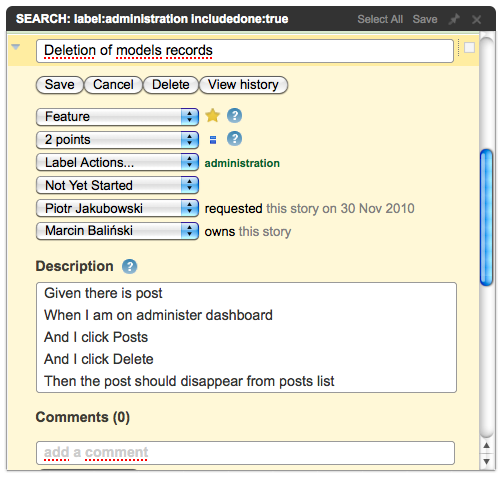
\includegraphics[width=\linewidth]{images/administer_story_desc.png}
  			\caption{Szczegółowy opis zadania}
  			\label{administer_story_desc}
  		\end{center}
  	\end{figure}
  	
  	\subsubsection{Czynności wstępne}
  	
  	Po zapoznaniu się i zrozumieniu istoty problemu, z którym będziemy się zmagać należy przygotować środowisko pracy. W naszym wypadku składają się na to dwie ważne czynności:
  	
  	 \begin{description}
        \item[Upewnienie się, że posiadamy aktualną wersję oprogramowania] Zawsze powinniśmy rozpocząć pracę z najnowszą rozwojową wersją kodu.
        \item[Uruchomienie pełnego zestawu testów] Przed rozpoczęciem pracy należy upewnić się, że wszystkie testy kończą się sukcesem.
      \end{description}
      
    Kod biblioteki administer przechowywany jest w rozproszonym systemie kontroli wersji GIT, spełnienie pierwszego punktu wymaga więc od programisty jedynie synchronizacji swojego lokalnego repozytorium z najnowszą wersją rozwojowej gałęzi kodu znajdującej się w głównym repozytorium. Szczegóły dotyczące operacji na systemie kontroli wersji wykraczają poza ramy tej pracy i zostaną tutaj pominięte. Przyjmijmy jednak, że synchronizacja została wykonana i mamy u siebie najnowszą wersję kodu biblioteki administer. 
    
    Uruchomienie pełnego zestawu testów daje nam pewność, że wersja oprogramowania, na której będziemy pracować spełnia warunki specyfikacji. Nie wolno rozpoczynać pracy jeśli testy z jakiegoś powodu nie przechodzą. W takim wypadku należy najpierw znaleźć przyczynę problemu i zlikwidować go a pracę nad nową funkcjonalnością rozpocząć dopiero kiedy wszystkie testy automatyczne sygnalizują sukces.
    
    Aby uruchomić pełen zestaw testów biblioteki administer wydajemy z głównego katalogu projektu polecenie:
    
    \begin{lstlisting}
      rake
    \end{lstlisting}
    
    Projekt został tak skonfigurowany, że komenda \verb+rake+ wywołana bez dodatkowych parametrów uruchamia zestaw scenariuszy Cucumber oraz testów RSpec opisujących zachowanie biblioteki. 
    
    
    
    \begin{figure}[!h]
  		\begin{center}
  			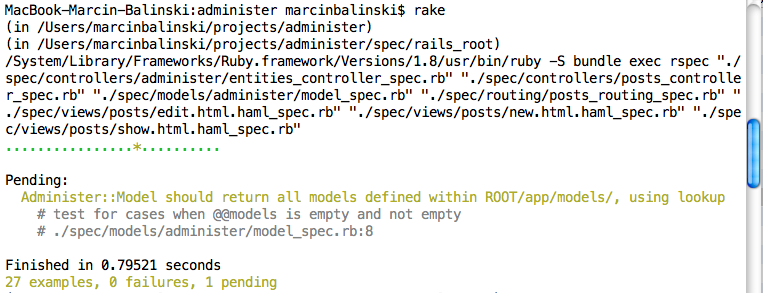
\includegraphics[width=\linewidth]{images/spec_report.png}
  			\caption{Zestaw testów RSpec - raport.}
  			\label{spec_report}
  		\end{center}
  	\end{figure}
  	
  	\clearpage
  	
  	\begin{figure}[!h]
  		\begin{center}
  			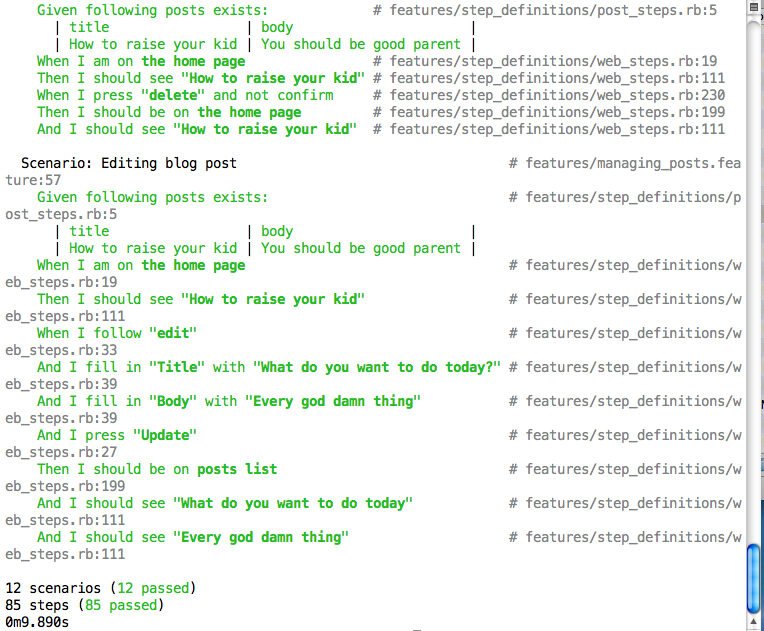
\includegraphics[width=\linewidth]{images/features_report.png}
  			\caption{Zestaw scenariuszy Cucumber - raport.}
  			\label{features_report}
  		\end{center}
  	\end{figure}
  	
  	  Raport po pozytywnym przejściu wszystkich testów powinien wyglądać podobnie jak na ilustracji \ref{spec_report} oraz \ref{features_report}. Oznaczenie \verb+pending+ przy jednym z testów RSpec sygnalizuje, że został tymczasowo wyłączony z zestawu testów przez jednego z programistów. Przyczyny wyłączenia testów mogą być różne, ale proceder ten należy stosować w ostateczności i w pełni świadomie, niedopuszczalne jest wyłączanie testu bez wyraźnego powodu a najlepiej jest, żeby takie sytuacje w ogóle się nie zdarzały.
  	  
  	\subsubsection{Więcej testów}
  	  Proces implementacji zaczyna się od stworzenia scenariusza opisującego nową funkcjonalność. W naszym przypadku scenariusze umieszczone są w podkatalogu \verb+spec/rails_root/features/+. Nas szczególnie interesuje plik \verb+spec/rails_root/features/administer/posts.feature+ w którym opisane jest zachowanie wymagane od panelu administrującego blogiem. W momencie pisania tego rozdziału plik \verb+posts.feature+ wygląda następująco:
  	  
  	\lstinputlisting{examples/code/ch04/02}
  	
  	Powyższe scenariusze opisują zachowanie biblioteki w tym momencie życia projektu, funkcja usuwania rekordu nie jest jeszcze opisana, nie pozostaje nam nic innego jak dopisać odpowiedni scenariusz:
  	
  	\lstinputlisting{examples/code/ch04/03}
  	
  	Oryginalny opis zadania (Ilustracja \ref{administer_story_desc}) został lekko zmodyfikowany w celu lepszego dopasowania do istniejącej infrastruktury i definicji kroków. Powtórne uruchomienie zestawu testów powinno zakończyć się niepowodzeniem - dodany przez nas scenariusz specyfikuje funkcjonalność, której jeszcze nie ma. Sytuację ilustruje zrzut ekranu \ref{scenario_failure}.
  	
  	\clearpage
  	
  	\begin{figure}[!h]
  		\begin{center}
  			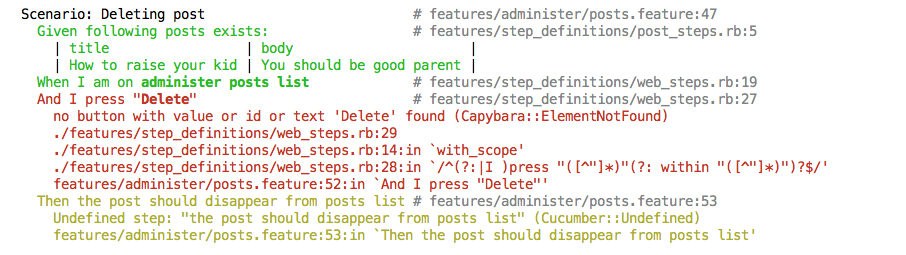
\includegraphics[width=\linewidth]{images/scenario_failure.png}
  			\caption{Nowo dodany scenariusz nie przechodzi}
  			\label{scenario_failure}
  		\end{center}
  	\end{figure}
  	
  	Oprócz informacji o błędzie, dostajemy również informacje o tym, że jeden z kroków scenariusza jest nie zdefiniowany:
  	
  	\begin{lstlisting}
    Undefined step: "the post should disappear from posts list" (Cucumber::Undefined)
    features/administer/posts.feature:53:in `Then the post should disappear from posts list'
    \end{lstlisting}
    
    Z problemem tym można poradzić sobie na dwa sposoby: dodać nową definicję dla kroku \verb+the post should disappear from posts list+ lub zmodyfikować scenariusz tak, aby korzystał z istniejących kroków nie zmieniając jednocześnie jego sensu. Generalnie rzecz biorąc niepotrzebne tworzenie nowych bytów nie jest dobrym pomysłem, należy przyjrzeć się więc czy możliwe jest wykorzystanie już istniejących definicji kroków, żeby opisać interesujące nas zachowanie. Plik
    
    \begin{lstlisting}
    spec/rails_root/features/step_definitions/post_steps.rb
    \end{lstlisting}
    
    definiuje następujące kroki:
    
    \lstinputlisting[language=ruby]{examples/code/ch04/05}
    
    Krok opisujący zniknięcie rekordu z listy można tak naprawdę opisać przy pomocy dwóch innych kroków, po pierwsze po kliknięciu przycisku \verb+Delete+ powinniśmy upewnić się, że nadal jesteśmy na liście Postów, po drugie wiedząc, że istniał tylko jeden post, po wciśnięciu \verb+Delete+ nie powinien istnieć żaden. Wykorzystamy więc dwa już zdefiniowane kroki: 
    
    \begin{lstlisting}
    I should be on administer posts list
    \end{lstlisting}
    
    oraz 
    
    \begin{lstlisting}
    there should be no posts
    \end{lstlisting}
    
    Zmodyfikowany scenariusz wygląda następująco:
    
    \lstinputlisting{examples/code/ch04/06}
    
    Powtórne uruchomienie testów nadal sygnalizuje niepowodzenie, jednak wszystkie kroki są zdefiniowane. Jedyne nad czym musimy się teraz skupić to dostarczenie funkcjonalności, która spełni warunki nowego scenariusza.
     
     \clearpage
     
     \begin{figure}[!h]
   		\begin{center}
   			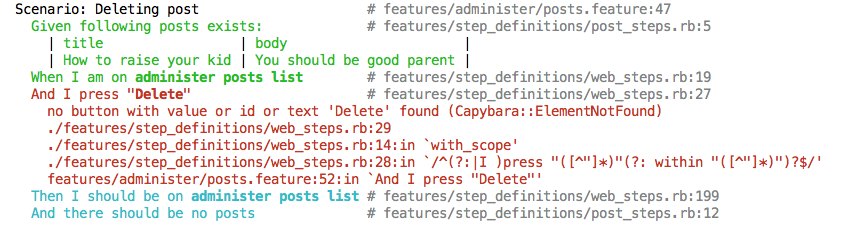
\includegraphics[width=\linewidth]{images/scenario_failure_2.png}
   			\caption{Nowo dodany scenariusz nie przechodzi, wszystkie kroki są zdefiniowane.}
   			\label{scenario_failure_2}
   		\end{center}
   	\end{figure}
   	
   \subsubsection{Dostarczenie wymaganej funkcjonalności}
   
   Nasze następne działania polegać będą na zaspokajaniu oczekiwań kolejnych kroków zdefiniowanego przez nas scenariusza aż do momentu ich wyczerpania i tym samym dostarczenia wymaganej funkcjonalności. Jak widać na ilustracji \ref{scenario_failure} dwa pierwsze kroki są zielone, skupmy się więc na trzecim z nich. Wszystko co musimy wiedzieć o przyczynach jego niepowodzenia zawarte jest w raporcie z przebiegu scenariusza:
   
   \begin{lstlisting}
   And I press "Delete"   # features/step_definitions/web_steps.rb:27
   
   no button with value or id or text 'Delete' found (Capybara::ElementNotFound)
   ./features/step_definitions/web_steps.rb:29
   ./features/step_definitions/web_steps.rb:14:in `with_scope'
   ./features/step_definitions/web_steps.rb:28:in `/^(?:|I )press "([^"]*)"(?: within "([^"]*)")?$/'
   features/administer/posts.feature:52:in `And I press "Delete"'
   \end{lstlisting}
   
   Przycisk \verb+Delete+ nie istnieje, dodajmy go do odpowiedniego widoku. Plik którego szukamy to 
   
   \begin{lstlisting}
   app/views/administer/entities/index.html.haml
   \end{lstlisting}
   
   Definiuje on widok panelu administracyjnego zobrazowany na ilustracji \ref{administer_index}
   
   \clearpage
   
    \begin{figure}[!h]
  		\begin{center}
  			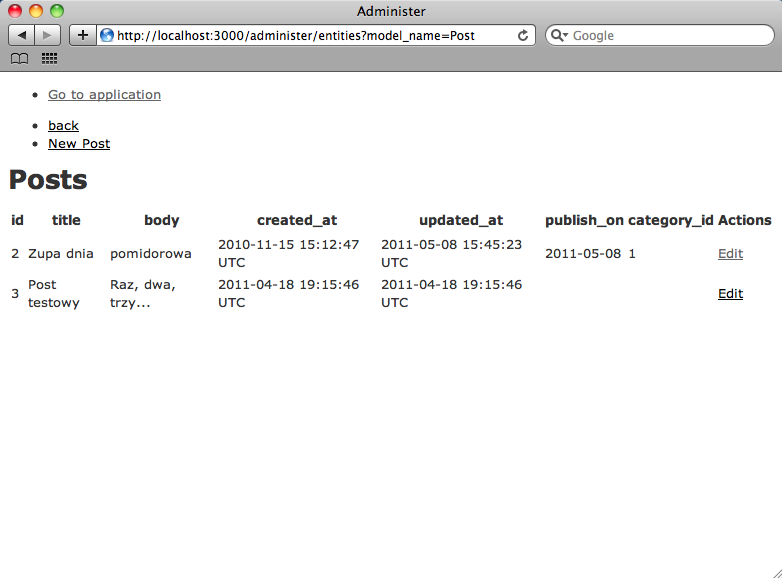
\includegraphics[width=\linewidth]{images/administer_index.png}
  			\caption{Lista rekordów wybranego modelu}
  			\label{administer_index}
  		\end{center}
  	\end{figure}
  	
  Jest to ten sam widok, o którym mowa w scenariuszu. Naszym zadaniem będzie dodać przycisk \verb+Delete+ w kolumnie \verb+Actions+ dla każdego wyświetlanego rekordu. Przyjrzyjmy się naszemu widokowi od środka:
  
  \lstinputlisting[numbers=left]{examples/code/ch04/07}
  
  Powyższy kod to prosty język szablonów HAML, który jest dynamicznie przetwarzany do postaci HTML zrozumiałej dla przeglądarki. Jeśli zlokalizujemy w nim kod odpowiedzialny za wyświetlenie linka \verb+Edit+ to prawdopodobnie bardzo łatwo będzie nam dodać pod nim przycisk \verb+Delete+. Interesujący nas fragment znajdziemy w 17 linii:
  
  \lstinputlisting[firstline=17,lastline=17]{examples/code/ch04/07}
  
  Modyfikujemy kod szablonu dodając brakujący przycisk, który połączony jest z akcją odpowiedzialną za usunięcie odpowiedniego rekordu. Po modyfikacji interesujący nas fragment kodu wygląda następująco:
  
  \lstinputlisting{examples/code/ch04/08}
  
  Dla zachowania poprawnej semantyki dokumentu dodanych zostało kilka tagów HTML, jednak najważniejsza deklaracja to:
  
  \lstinputlisting[firstline=4,lastline=4]{examples/code/ch04/08}
  
  Kod ten składa się z metod implementowanych przez framework Rails oraz metod specyficznych dla samego projektu administer. W wyniku jego działania wygenerowany zostanie przycisk o etykiecie \verb+Delete+ powiązany z metodą \verb+destroy+ kontrolera, który odpowiedzialny jest za zarządzanie rekordami modeli biznesowych przez bibliotekę administer. W kontekście naszych rozważań na temat testowo zorientowanych metod rozwoju oprogramowania istotne jest, że modyfikacja ta zaspokaja wymaganie kroku scenariusza, nad którym aktualnie pracujemy. Uruchommy ponownie zestaw testów, aby przekonać się, że mimo iż przycisk \verb+Delete+ w tej chwili istnieje, to jednak ciągle są problemy z tym samym krokiem, informacja o niepowodzeniu jest jednak inna niż poprzednio:
  
  \begin{lstlisting}
  And I press "Delete"  # features/step_definitions/web_steps.rb:27
  
  The action 'destroy' could not be found for Administer::EntitiesController (AbstractController::ActionNotFound)
  ./features/step_definitions/web_steps.rb:29
  ./features/step_definitions/web_steps.rb:14:in `with_scope'
  ./features/step_definitions/web_steps.rb:28:in `/^(?:|I )press "([^"]*)"(?: within "([^"]*)")?$/'
  features/administer/posts.feature:52:in `And I press "Delete"'
  \end{lstlisting}
  
  Wyświetlamy przycisk \verb+Delete+ oraz jest on prawidłowo skojarzony z akcją \verb+destroy+ kontrolera \verb+Administer::EntitiesController+. Problem w tym, że akcja \verb+destroy+ nie została jeszcze zaimplementowana co skutkuje błędem - próbą uruchomienia nieistniejącej akcji w momencie kiedy użytkownik (W tym wypadku symulowany przez bibliotekę Capybara) klika w przycisk.
  
  Przejdźmy więc do wyżej wymienionego kontrolera \verb+EntitiesController+. Jego głównym zadaniem jest obsługa żądań związanych z modelami biznesowymi istniejącymi w aplikacji, która korzysta z biblioteki administer do zadań tych zaliczają się m.in dodawanie, modyfikowanie i usuwanie rekordów tych modeli. Pełen kod kontrolera wygląda w tym momencie następująco:
  
  \lstinputlisting[language=ruby]{examples/code/ch04/09}
  
  Kontroler ten definiuje akcje, które użytkownik może za jego pomocą wykonać, oprócz tego robi kilka innych ciekawych rzeczy. Przede wszystkim ustala informację o rodzaju modelu, na którym ma przeprowadzać operacje. Nazwa modelu jest przekazywana jako jeden z parametrów żądania (\verb+params[:model_name]+) i to na jej podstawie znajdowana jest właściwa klasa reprezentująca ten model, konkretne jego rekordy, lub cała ich kolekcja.
  W tej chwili istnieją cztery akcje: \verb+new+, \verb+create+, \verb+edit+ oraz \verb+update+ brakuje (o czym zostaliśmy już poinformowani przez nieprzechodzący scenariusz) akcji \verb+destroy+, której implementacją zajmiemy się w tej chwili.
  
  Z treści naszego scenariusza wynika, że zadaniem akcji \verb+destroy+ jest usunięcie konkretnego rekordu z bazy danych oraz przekierowanie użytkownika z powrotem na listę wszystkich rekordów. Na wejściu akcja musi więc otrzymać dwa parametry: nazwę modelu oraz identyfikator rekordu a na podstawie tych danych wykonać polecenie które usunie rekord należący do tego modelu oraz noszący taki właśnie identyfikator. Kod spełniający taką specyfikacje może wyglądać następująco: 
  
  \lstinputlisting[language=ruby,numbers=left]{examples/code/ch04/10}
  
  Po dodaniu metody \verb+destroy+ do kontrolera uruchamiamy testy raz jeszcze przy pomocy polecenia \verb+rake+. Tym razem wszystkie scenariusze przechodzą.
  
  \clearpage
  
   \begin{figure}[!h]
 		\begin{center}
 			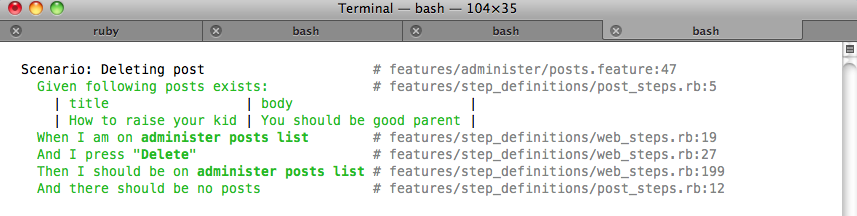
\includegraphics[width=\linewidth]{images/delete_record_scenario_pass.png}
 			\caption{W tym momencie funkcjonalność spełnia wymagania scenariusza.}
 			\label{delete_record_scenario_pass}
 		\end{center}
 	\end{figure}
 	
 	Teoretycznie moglibyśmy w tym momencie uznać zadanie za zakończone, jednak pisząc metodę \verb+destroy+ wykroczyliśmy nieco poza to, co opisane zostało w scenariuszu, linie 3-5 definiują następujący blok kodu:
 	
 	\lstinputlisting[language=ruby,firstline=3,lastline=5]{examples/code/ch04/10}
 	
 	Jeśli usunięcie rekordu z jakiejś przyczyny nie zakończy się powodzeniem wyświetlony zostanie komunikat o treści:
 	
 	\begin{lstlisting}
 	Could not destroy object.
 	\end{lstlisting}
 	
 	Zachowanie to jest jak najbardziej sensowne, zostało ono jednak dodane samowolnie i nie jest nigdzie przetestowane. Jako odpowiedzialni programiści nie powinniśmy dopuścić do takiej sytuacji i dopisać odpowiedni test. Przetestowanie tego zachowania scenariuszem Cucumber jest trudne, trudno bowiem odtworzyć sytuację, w której usunięcie rekordu zakończy się niepowodzeniem - może się tak stać np. kiedy silnik bazy danych w której jest przechowywany nałożył na ten rekord blokadę, która trwa w momencie próby jego usunięcia. W tej sytuacji do testowania wykorzystamy bibliotekę RSpec i jej mechanizm oczekiwań oraz sztucznych obiektów. Odpowiedni zestaw testów zdefiniowany jest w pliku:
 	
 	\begin{lstlisting}
 	spec/rails_root/spec/controllers/administer/entities_controller_spec.rb
 	\end{lstlisting}
 	
 	W którym następująco opiszemy interesujące nas zachowanie:
 	
 	\lstinputlisting[language=ruby]{examples/code/ch04/12}
 	
 	Upewniliśmy się, że informacja o błędzie została ustawiona w kontrolerze. To jednak nie wszystko, musimy sprawdzić, czy jest ona wyświetlona w odpowiednim widoku. Administer wyświetla informacje o błędach w głównym widoku zdefiniowanym w pliku:
 	
 	\begin{lstlisting}
 	app/views/layouts/administer.html.haml
 	\end{lstlisting}
 	
 	Odpowiedni test ma sprawdzać, czy ustawiony komunikat zostanie wyświetlony:
 	
 	\lstinputlisting[language=ruby]{examples/code/ch04/13}
  
  \section{Wnioski}

\end{document}
